%
% File coling2020.tex
%
% Contact: feiliu@cs.ucf.edu & liang.huang.sh@gmail.com
%% Based on the style files for COLING-2018, which were, in turn,
%% Based on the style files for COLING-2016, which were, in turn,
%% Based on the style files for COLING-2014, which were, in turn,
%% Based on the style files for ACL-2014, which were, in turn,
%% Based on the style files for ACL-2013, which were, in turn,
%% Based on the style files for ACL-2012, which were, in turn,
%% based on the style files for ACL-2011, which were, in turn, 
%% based on the style files for ACL-2010, which were, in turn, 
%% based on the style files for ACL-IJCNLP-2009, which were, in turn,
%% based on the style files for EACL-2009 and IJCNLP-2008...

%% Based on the style files for EACL 2006 by 
%%e.agirre@ehu.es or Sergi.Balari@uab.es
%% and that of ACL 08 by Joakim Nivre and Noah Smith

\documentclass[11pt]{article}
\usepackage{coling2020}
\usepackage{times}
\usepackage{amsmath,amsfonts,amssymb}
\usepackage{url}
\usepackage{latexsym}
\usepackage{hyperref}
\usepackage[noabbrev,capitalize]{cleveref}
\usepackage{graphicx}
\usepackage{natbib}
\usepackage{pgfplots}

%\setlength\titlebox{5cm}
%\colingfinalcopy % Uncomment this line for the final submission

% You can expand the titlebox if you need extra space
% to show all the authors. Please do not make the titlebox
% smaller than 5cm (the original size); we will check this
% in the camera-ready version and ask you to change it back.


\title{Composing Byte-Pair Encodings for Morphological Sequence Classification}


\author{Adam Ek \and Jean-Philippe Bernardy\\
	Centre for Linguistic Theory and Studies in Probability,\\
	Department of Philosophy, Linguistics and Theory of Science,\\
	University of Gothenburg,\\
	\texttt{adam.ek@gu.se}}

\date{}

\begin{document}
	\maketitle
	
	\begin{abstract}
		This document contains the instructions for preparing a paper submitted
		to COLING-2020 or accepted for publication in its proceedings. The document itself
		conforms to its own specifications, and is therefore an example of
		what your manuscript should look like. These instructions should be
		used for both papers submitted for review and for final versions of
		accepted papers. Authors are asked to conform to all the directions
		reported in this document.
	\end{abstract}
	
	\section{Introduction}
	\label{intro}
	
	\textbf{Things added to model:}
	\begin{itemize}
		\item Adaptive learning rate
		\item Fine-tuning
		\item Dropouts
		\item Trained character representations (?)
	\end{itemize}
	
	\textbf{Things to add:}
	\begin{itemize}
		\item (results) More detailed accuracy for len(BPE)$>2$
		\item (results) With fine-tuning/without fine-tuning
		\item (data) Data statistics: number of MSD-tags 
		\item (data) Pick other datasets, try to match dataset sizes better (100k-150k train examples, turkish very small atm)
	\end{itemize}

        Since its introduction \cite{todo}, the transformer model has
        emerged as the dominant architecture for statistical language
        model, gradually displacing recurrent neural networks, in
        particular the LSTM and its variants. The transformer owes its
        success to several factors, including the availability of
        pretrained models, which effectively yield rich contextual
        word embeddings. Such embeddings can be used as is (for
        so-called feature extraction), or the pre-trained models can
        be fine-tuned to specific applications.

	At the same time as transformer models became popular, the
        tokenization of natural language texts have shifted away from
        methods explicitly oriented on words or morphemes. Rather,
        statistical approaches are favoured to splits strings of
        characters into units which are not necessarily meaningful
        linguistically, but rather have statistically balanced
        frequencies. For example, the word "scientifically" may be
        composed of the tokens: "scient", "ifical", "ly" --- here the
        central token does not correspond to a morpheme.
        %
        Rather than identifying complete words or morphemes, it aims
        to find sub-word units occurring significantly often. Typical
        approaches to composing tokens from sub-token units have
        focused on combining character n-grams \cite{TODO:bojanowski},
        while other approaches have looked at splitting words into
        \textit{roots} and \textit{morphs}\jp{morphemes?}, and then
        combining them. In this paper, we consider in particular
        Byte-Pair Encodings (BPE) \citep{sennrich2015neural}, which take another approach. One does not
        specifically look for either character n-grams or morphs, but
        rather it aim to split a corpus $\mathcal{C}$ into $N$ tokens,
        where $N$ is user defined. [EXPAND]

        One issue with statistical tokenization is that one is seldom
        interested in the encoding, but rather in the semantically
        meaningful units in the original texts. Thus the question of
        mapping data about the token back to the original text arises.

	In this paper we explore how to combine Byte-Pair Encodings
        from a transformer model to perform sequence
        classification, which is used in particular in the popular BERT model \citep{devlin2018bert}. For our purposes, the goal in sequence
        classification is to assign a label to every word in a
        sentence. When we are using byte-pair encoding (or similar
        sub-token representations) we must then find some way of
        combining the units that build the word, before it is
        eventually assigned a label. Coming back to our example, we
        must map the feature-set assigned (depending on the context)
        to "scient", "ifical", "ly". Then this combined feature set is
        mapped to a class for the whole word ``scientifically''.

	To our knownledge, this is a little studied
        problem. \citet{todo} have only brushed the surface by
        reporting that few differences are found between different
        methods. In this paper we wish to explore the problem in
        further detail and identify what effect different methods have
        on the final performance of a model.

    %In this paper we explore the transformer model applied to sequence classification. In sequence classification a dataset is split into words (or tokens) and each word is assigned a label. 
    %Neural model can predict the label of a word by assigning it a representation and passing it through the network. However, the transformer model use byte-pair encoding (BPE) \cite{sennrich2015neural}, or some variation of it \citep{devlin2018bert}, to tokenize text. 
    %BPE tokens are sub-strings that occur significantly often in the corpus, and does not correspond directly to words. 
    %
    %In sequence classification, we need to assign a label to the word "scientifically". But the word is now composed of three BPE embeddings, so to predict a label for the word we need to compose all of the BPE embeddings into one representation.
    
    %In this project is to explore six different methods of creating word representations from multiple BPE embeddings.
	
%%%
    %Typically, the transformer model use some variation of byte-pair endings (BPE)  to split sentences into tokens. For non-bpe tokenization schemas typically words are selected based on white-space. This is convenient in sequence classification or parsing where for each word some label is assigned. 
    %In the BPE schema on the other hand a word (which has a label attached to it in some dataset) may be split into two or more BPE-tokens. 
    %The BPE vocabulary is usually selected such that significantly common sub-strings are saved. To create words using a BPE vocabulary, sub-strings are combined with each other.
    
    %In this project we explore how to compose embeddings of BPE tokens into word representations. More specifically, in cases when a word is associated with several BPE embeddings (for example: the word "scientifically" may be composed of the the BPE tokens: ["scient", "ifical", "ly"]) how do we combine the BPE embeddings to create a word representation ("scientifically") which we assign a label to.
    
    %\paragraph{Task:} We explore combination of BPE embeddings with the task of Morphological-Tagging-in-Context \citep{mccarthy2019sigmorphon}. 
    %The task is simply to predict the morphological features (such as case, number person, ...) of each word (as defined in the dataset) given the sentence which the word occur in.
    
    \paragraph{Task:} In this paper we explore morphological sequence classification. Morphological tagging involves identifying a set of morphological features that a word posses, such as number, person, case and so on. 
    Morphological features primarily depend on the affixes of words, but additional information is also provided by the words context. 
    
    \paragraph{Data:} For the task we will use the Universal Dependencies dataset \citep{nivre2018} annotated with the UniMorph schema \citep{mccarthy2018marrying}. We are interested both in the general effects of using different composition methods, and whether some methods favor languages with certain typology. To explore this, we take a sample of eight languages from the Universal Dependencies dataset, four languages that use \textit{fusional} morphology, an affix may be indicative of one or more morphological features, and four languages that use \textit{agglutinative} morphology, each affix is mapped to one and only one morphological feature. 
    
   	The fusional languages we look at are Arabic, Czech, Polish and Spanish, and the agglutinative languages we look at are Finnish, Basque, Turkish and Estonian. The size of the dataset and the average number of BPE tokens per word are shown in \cref{tab:data}.
    
    	\begin{table}[h]
		\centering
		\begin{tabular}{l|lrrrr}
			Language & Typology & $\frac{BPE}{word}$ & Train & Validation & Test \\
			\hline
			Arabic-PADT  & Fusional & 1.39 & 225494 & 28089 & 28801  \\
			Czech-CAC   & Fusional & 1.77 & 395043 & 50087 & 49253 \\
			Polish-LFG & Fusional & 1.75 & 104730 & 13161 & 13076 \\
			Spanish-AnCora & Fusional & 1.34 & 439925 & 55196 & 54449 \\
			Finnish-TDT & Agglutinative & 1.98 & 161791 & 19876 & 20541 \\
			Basque-BDT  & Agglutinative & 1.79 & 97336 & 12206 & 11901 \\
			Turkish-IMST & Agglutinative & 1.73 & 46417 & 5708 & 5734 \\
			Estonian-EDT & Agglutinative & 1.86 & 346986 & 43434 & 43825 \\
		\end{tabular}
		\caption{\label{tab:data} Treebank statistics.}
	\end{table}
    
    The fusional languages where chosen such that two of them (Czech and Polish) have a higher BPE per token ratio than the other two (Arabic and Spanish). We do this because one factor that impact composition method may be BPE per token ratio, and we want to exclude this from our analysis. Thus, by having both fusional and agglutinative languages with similar BPE per token ratio we can discard this as an explanatory factor. 
    

	
	\section{Method}
	\label{method}
	
	In this section we present the model used for sequence classification, the methods we use to compose BPE embeddings, and how we trained the model.
	
	
	\paragraph{Transformer model}
	For the task we use the XLMR \citep{conneau2019unsupervised} model\footnote{We use the huggingface implementation [CITE/LINK]}. XLMR is a masked language model based on the transformer (specifically, RoBERTa \citep{liu2019roberta}) trained on data from 100 different languages, using a shared vocabulary. In this experiment we use \textsc{XLMR}$_{base}$ model, it has 12 encoder layers, 16 (?) attention heads and use 768 dimensions for its hidden size. 
	
	\subsection{Byte-pair combination methods}
	


	
	\subsection{Model}
	For morphological tagging we use the XLMR base model with a classification module on top. The classification module is a LSTM followed by a two layer linear transformation. 
	
	The model we use to predict morphological features is simple. For each sentence we extract $n$ BPE embeddings from $XLMR_{base}$ then align them to words. 
	We then run all words who consist of more than one BPE embedding through a function $f$ which combine the BPE embeddings. This produce one embedding per word which we concatenate with character features generated by a character LSTM. We then pass the BPE features concatenated with the character features to a LSTM to extracxt contextual features.
	We pass the LSTM outputs to a linear transformation layer that compute scores for each class in the output. We then apply softmax and compute the loss.
	
	An outline of the model is presented in \cref{fig:model}, in the outline $f$ represent the different methods we use to combine BPE embeddings.
	
	\begin{figure}[h!]
		\centering
		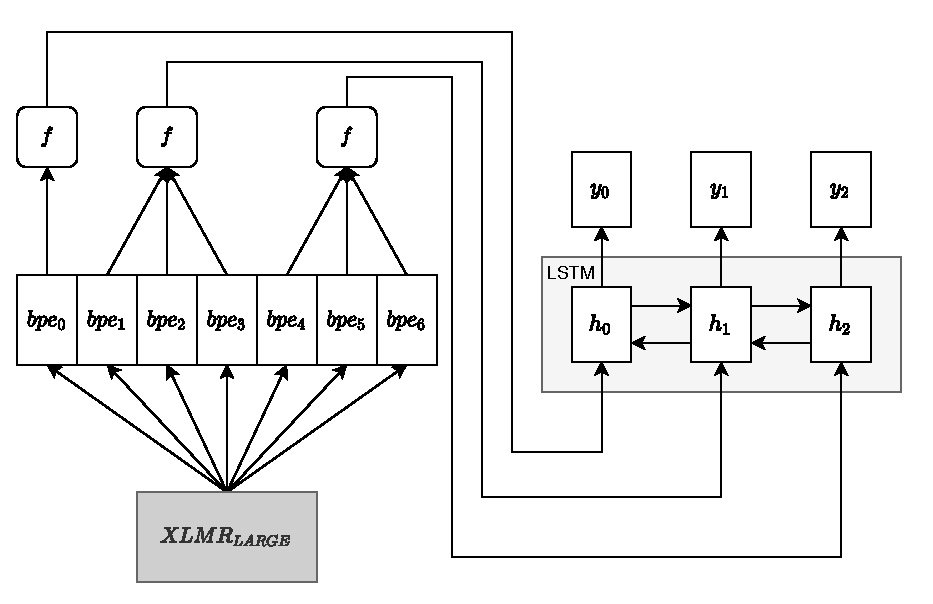
\includegraphics[scale=0.2]{model_outline-5.pdf}
		\caption{\label{fig:model} Procedure outline}
	\end{figure}
	
	\subsubsection{BPE features} 	
	
	We obtain BPE features for a \textit{token} by combining the BPE tokens that compose the token by combining their features using three different methods:
	
	\paragraph{Sum:} For the sum method, we take the sum for each dimension of all BPE embeddings. Thus, for dimension $i$ we add all the values in all BPE embeddings $x_i^0 + ,..., + x_i^n$:
	
	\begin{equation}
	x'_{i} = \sum_{j=1}^{n} x_i^j
	\end{equation}
	
	
	\paragraph{Mean:} In the mean method we calculate the sum and divide by the number of BPE embeddings in the word. Thus, for dimension $i$ we calculate $\frac{x_i^0 + ,..., + x_i^n}{n}$: 
	
	\begin{equation}
	x'_{i} = \frac{1}{n}\sum_{j=1}^{n} x_i^j
	\end{equation}
	
	
	\paragraph{RNN:} In this method we employ a bidirectional RNN to learn how to compose the BPE embeddings. For each multi-BPE token, we pass the sequence of BPE embeddings through an RNN and use the final output as the word representation.
	
	\subsubsection{XLMR features}
	
	When extracting features from XLMR we compute a weighted sum of the layer representations. This is inspired by previous work showing that the different layers in language models encode different kinds of information. That is, we create a random vector $w$ with one element per layer, indicating the importance of the layer. We calculate the layerwise weighted sum for each bpe representation as follows:
	
	\begin{equation}
		x_i = \sum_{1}^{J} softmax(c)_j l_{ji}
	\end{equation}
	
	\subsubsection{Character features}
	In addition to layer attention we use a character LSTM to extract a word representation based on characters. The final representation we pass to the word-LSTM is the concatenation of the word representation based on BPE compositions and characters, $w_i = \text{concat}(f(bpe_0,...,bpe_K), LSTM(c_0, ..., c_M))$
	
	\subsubsection{Label smoothing}
	Given that many of the languages have a large number of morphological tags we want to prevent the model from growing overconfident for certain classes. To address this we introduce label smoothing, that is, instead of the incorrect classes having 0 probability and the correct class $100\%$ probability we let each of the incorrect classes have a probability of $\alpha$. We assign probabilities to a target $t$ by $(1-\alpha)t + \alpha / |C|$ where $|C|$ is the number of classes. 
	

	
	\subsection{Training}
	
	When fine-tuning the model we freeze the XLMR parameters for the first epoch.
	When training the model we use cosine annealing learning rate with restarts every epoch, that is, the learning rate starts high then incrementally decrease to $1e-12$ during N steps, where N is the number of batches in an epoch.
	
	\begin{table}[h]
		\centering
		\begin{tabular}{lr}
			Parameter & Value \\
			\hline
			Epochs & 15 \\
			Batch size & 4 / 32 \\
			Character representation size & 128 \\
			% optimizers
			Optimizer & Adam \\
			Learning rate & 0.001 \\
			Learning rate$_{xlmr}$ & 1e-06 \\
			% regularization
			Label smoothing & 0.03 \\
			
		\end{tabular}
		\caption{\label{tab:parameters} Hyperparameters used for training the model. Slashed indicate the value of a parameter when we finetune or extract features.}
	\end{table}

	
	\section{Results}
	\label{results}
	
	
	
	We present the accuracy of assigning morphological tags to all tokens in \cref{tab:results_tokens}. Both when we finetune and only extract BPE weights we see that using an RNN to compose BPE tokens yields slightly better performance.
	%
	In general, our results are lower than the reported State-of-the-Art.
	

	\begin{table}[h]
	%\small
	\centering
	\begin{tabular}{l|c|ccc|ccc}
		& & \multicolumn{3}{c}{Finetuning} & \multicolumn{3}{c}{Feature extraction} \\
		Treebank & Baseline & Sum & Mean & RNN & Sum & Mean & RNN \\
		\hline
		% agglutinative languages
		Finnish-TDT & .751 & .965 & .963 & \textbf{.967} & .930 & .931 & \textbf{.942} \\ 
		Basque-BDT & .676 & .910 & .909 & \textbf{.920} & .865 & .865 & \textbf{.888} \\
		Turkish-IMST & .620 & .898 & .891 & \textbf{.905} & .856 & .849 & \textbf{.866}\\
		Estonian-EDT & & & & & .931 & .934 & \textbf{.939} \\
		% fusional languages
		Spanish-AnCora & .842 & .979 & .979 & \textbf{.980} & .968 & .967 & \textbf{.971} \\
		Arabic-PADT & .770 & .952 & .953&\textbf{.954} & .941 & .939 & \textbf{.948} \\
		Czech-CAC & .771 &  &  &  & .944 &  &  \\
		Polish-LFG & & & &  & .907 & .907 & \textbf{.928} \\
	\end{tabular}
	\caption{\label{tab:results_tokens} Accuracy for morphological tagging. We evaluate both when we finetune the XLMR model and when we only extract BPE embeddings weights.}
	\end{table}

	However, the results in \cref{tab:results_tokens} also include tokens which are only composed of one BPE token. To better evaluate our composition methods we compute the accuracy for tokens which are composed of two or more BPE tokens. The results can be seen in \cref{tab:results_large_tokens}.

	\begin{table}[h]
	%\small
	\centering
	\begin{tabular}{l|ccc}
		 & \multicolumn{3}{c}{Method} \\
		Treebank & Sum & Mean & RNN \\
		 		\hline
		% agglutinative languages
		Finnish-TDT & .893 & .897 & \textbf{.913} \\ 
		Basque-BDT  & .802 & .803 & \textbf{.840} \\
		Turkish-IMST & .807 & .796 & \textbf{.816} \\
		Estonian-EDT & .904 & .908 & \textbf{.916} \\
		% fusional languages
		Spanish-AnCora & .952 & .951 & \textbf{.959} \\
		Arabic-PADT & .927 & .925 & \textbf{.935}\\
		Czech-CAC & & & \\
		Polish-LFG & .834 & .833 & \textbf{.876} \\
	\end{tabular}
	\caption{\label{tab:results_large_tokens} Accuracy for morphological tagging on all tokens that are composed of 2 or more BPE tokens.}
\end{table}

\begin{center}
	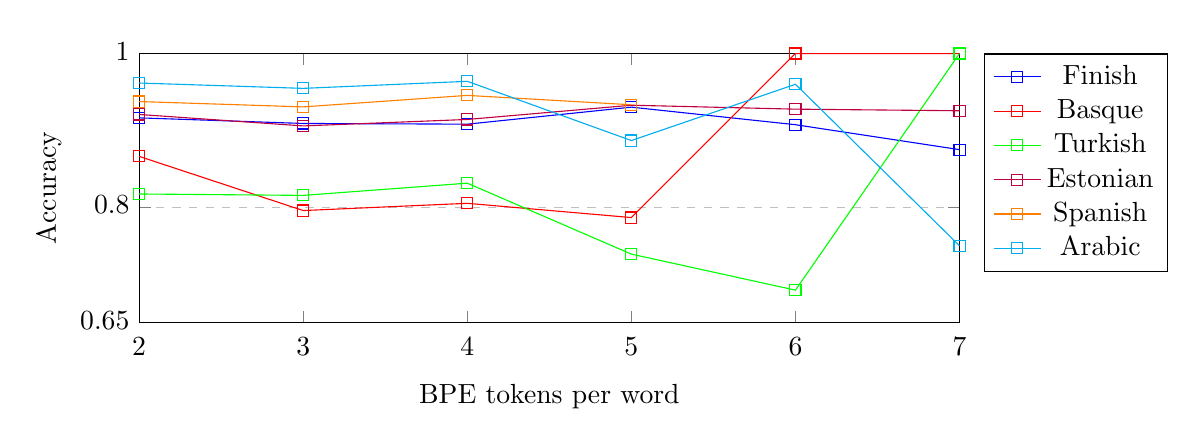
\begin{tikzpicture}

	\begin{axis}[
	title={},
	xlabel={BPE tokens per word},
	ylabel={Accuracy},
	xmin=2, xmax=7,
	ymin=0.65, ymax=1,
	xtick=data,
	ytick={0.65,0.8,1.0},
	typeset ticklabels with strut,
	legend pos=outer north east,
	ymajorgrids=true,
	grid style=dashed,
	width=12cm,
	height=5cm
	]
	
	\addplot[
	color=blue,
	mark=square,
	]
	coordinates {(2, 0.9163053722902922)(3, 0.9090291921249152)(4, 0.9081133919843597)(5, 0.9302325581395349)(6, 0.9074074074074074)(7, 0.875)};
	\legend{Finnish}
	
	\addplot[
	color=red,
	mark=square,
	]
	coordinates {(2, 0.8662081900593935)(3, 0.7957794417971409)(4, 0.8051948051948052)(5, 0.7866666666666666)(6, 1.0)(7, 1.0)};
	\legend{Basque}
	
	\addplot[
	color=green,
	mark=square,
	]
	coordinates {(2, 0.8173395102581072)(3, 0.8154981549815498)(4, 0.8313953488372093)(5, 0.7391304347826086)(6, 0.6923076923076923)(7, 1.0)};
	\legend{Turskish}
	
	\addplot[
	color=purple,
	mark=square,
	]
	coordinates {(2, 0.9207130730050934)(3, 0.9058250456667343)(4, 0.9142367066895368)(5, 0.9327433628318584)(6, 0.9276315789473685)(7, 0.925531914893617)};\legend{Estonian}
	
	\addplot[
	color=orange,
	mark=square,
	]
	coordinates {(2, 0.9375252729478366)(3, 0.930576070901034)(4, 0.9455252918287937)(5, 0.9333333333333333)};\legend{Arabic}
	
	\addplot[
	color=cyan,
	mark=square,
	]
	coordinates {(2, 0.9616295004360284)(3, 0.9546589018302829)(4, 0.9638242894056848)(5, 0.8867924528301887)(6, 0.96)(7, 0.75)};\legend{Spanish}
	
	\legend{
		Finish,
		Basque,
		Turkish,
		Estonian,
		Spanish,
		Arabic
	}
	
	\end{axis}
	\end{tikzpicture}
\end{center}

	
	
	\section{Discussion}
        %We can observe an interesting trend for the treebank samples. For the languages with agglutinative morphology\footnote{1-to-1 correspondence between morphemes and grammatical/syntactic features.} the average increase using RNN compared to Mean is 4.3\%. For the fusional\footnote{1-to-many correspondence between morphemes and grammatical/syntactic features.} languages, the difference between RNN and Mean is only 1.1\%. 
        
        %Interestingly, this observation seem task-dependant rather than BPE dependant. We can see in \cref{tab:data} that Czech is a fusional language, but with a BPE-to-word ratio ($1.77$) comparable to the agglutinative languages. But, Czech also exhibit the pattern of benefiting less from RNN than from Mean, indicating that fusional languages\footnote{In our language/treebank sample.} regardless of BPE-to-word ratio is less affected by the composition method than agglutinative languages. 
        
        %In general, the agglutinative languages have a higher BPE-to-word ratio, with one exception, Czech. Czech have a BPE-to-word ratio of $1.77$, but still exhibit a lower difference between the RNN and mean method. Thus, from this small sample of treebanks it appears as if the method of combining BPE embeddings is more important for agglutinative languages than for fusional languages. 
        
        Analogously to character embeddings, the RNN method seem to provide stronger results than using either Sum or Mean for combining BPE tokens. We hypothesize that this is because Sum or Mean don't respect the ordering of elements within a word, that is, we don't relate the values of $BPE_0$ to $BPE_{1:N}$ with respect to the morphological tags. 
    
    \section{Conclusions}
    	As a general summary of our work, we highlight that language typology is not irrelevant when working with models that employ byte-pair encoding.     
	
	%\section*{Acknowledgments}
	
	
	% include your own bib file like this:
	\bibliographystyle{plain}
	\bibliography{coling2020}
	
\end{document}
